\section{案例研究与性能评估}
\label{sec:experiments}

\subsection{数据集与实验设置}
\label{subsec:exp_setup}

为了验证所提出的 PhysFormer 架构，我们在一套高保真虚拟电厂（VPP）数据集上进行了广泛的实验，该数据集由德国某分布式能源集群的区域测量聚合而成。数据集捕获了连续 3 年（2012--2014 年）内太阳能光伏发电、风力发电和商业电力负荷的详细 15 分钟分辨率轨迹，共计 105,120 个采样间隔。数据按时间顺序划分为训练集（70\%）、验证集（10\%）和测试集（20\%）。为了在保持物理边界的同时维持数值稳定性，所有输入特征均使用全局 Z-score 参数（$\mu, \sigma$）进行标准化，这些参数被显式记录用于 BPAR 层中的物理重投影。模型超参数配置为与现代基准模型相当的复杂度：隐藏层维度 $d_{\text{model}} = 512$，前馈维度 $d_{\text{ff}} = 1024$，自注意力头数 $n_{\text{heads}} = 8$，以及层数 $e_{\text{layers}} = 3$。为了评估计算效率，我们在等效的隐藏维度 $d_{\text{model}} = 512$ 下将 PhysFormer 与 Informer 进行了基准测试。PhysFormer 包含 $11.4$M 个参数，显着低于 Informer 的 $17.9$M 个参数，验证了其双流架构的归纳效率。在 NVIDIA RTX 3090 GPU 上测得的推理延迟为 $2.10$~ms/样本（批大小为 1），模拟了 VPP 调度的实时滑动窗口更新。

我们将 PhysFormer 与八个极具竞争力的基准模型进行了比较：标准循环网络（LSTM、GRU）、物理信息神经网络（PINN）\cite{Raissi2019}，以及先进的时间序列 Transformer 架构，包括 Informer \cite{Zhou2021informer}、Autoformer \cite{Wu2021autoformer}、PatchTST \cite{Nie2023patchtst}、DLinear \cite{Zeng2023}，以及最先进的 iTransformer \cite{Liu2023itransformer}。为了保证绝对公平的评估，结构相同的未来天气协变量（$\mathcal{X}_{\text{weather\_future}} \in \mathbb{R}^{B \times P \times 3}$）被统一提供给了所有参与对比的基线模型。对于 Transformer 基准模型，这些外源变量被严格拼接到它们标准的解码器嵌入结构中，并以等效的动态协变量形式提供给循环模型。因此，PhysFormer 所展现出的预测优势根本上源自其机制性的物理引导架构（例如在消融实验中评估的特定的 Future GLU 注入路径），而不是来自对未来大气数据的不对称获取。

为了全面评估预测性能，我们采用了六个不同的指标。标准准确性指标包括均方误差（MSE）、平均绝对误差（MAE）和均方根误差（RMSE）。除标准准确性外，我们正式定义了三个物理合规性指标：边界违规率（BVR）、平均违规严重程度（MVS）和爬坡违规指标（RVM）。BVR 测量违反已知物理限制（例如负发电功率）的预测百分比。为了量化这些违规的严重程度，MVS 被正式定义为落在可行物理边界之外的预测值的平均绝对大小。除了静态边界外，我们还通过爬坡违规指标（RVM）及其发生频率（爬坡违规率 RVR）来评估时间一致性。最后，净平均绝对误差（NET MAE）被正式定义为预测的聚合组件与真实值净需求之间的平均绝对不平衡量，即 $\text{mean}(|\sum_c \hat{y}_c - y_{\text{net}}|)$。每个通道的爬坡阈值 $\rho_k$ 被凭经验确定为训练集差异的第 $99.9$ 百分位移，而“严格”阈值（RVR-S）设定在第 $99.5$ 百分位移且不带安全因子，以捕获高频伪影。

\subsection{预测性能分析}
\label{subsec:performance}

全球测试集上的主要预测结果见表~\ref{tab:main_results}。在同类竞争模型中，PhysFormer 实现了 $0.0128$ 的 MSE，与不受约束的 SOTA 基准模型（Informer 为 $0.0121$，iTransformer 为 $0.0122$）相比，其误差保持在 $6\%$ 以内。虽然这些模型通过复杂的注意力机制优先考虑统计曲线拟合，但它们遭受严重的物理合规性缺陷，其中 iTransformer 的边界违规率（BVR）峰值达到 $16.26\%$。此外，我们强调了一个关于时间连续性的关键“安全优先权衡”。在严格阈值下，iTransformer 的 RVR-S 为 $0.028\%$，而 PhysFormer 为 $0.198\%$。然而，不受约束模型的这种“平滑性”往往是以牺牲物理有效性为代价实现的；它们之所以能保持连续轨迹，正是因为它们忽视了物理零边界。PhysFormer 的 $0.198\%$ RVR-S 代表了其 BPAR 机制为确保绝对安全（BVR=0.00\%）而在物理边界处进行的必要结构修正。至关重要的是，这些修正的绝对量阶（RVM-Mag）保持在 $2.6 \times 10^{-5}$ MW 级别，证明了 PhysFormer 通过优先考虑绝对物理安全而非表面的平稳性，成功解决了这一权衡。

有趣的是，像 PatchTST 和 DLinear 这样独立于通道的模型在这种特定的 VPP 设置下表现出通道独立的失败，其表现不如性能更强的多变量模型。这强调了对多源能源系统固有的密集跨通道依赖性进行建模的必要性。同时，PINN 的结构优势显而易见；其物理归纳偏向帮助其超越了标准的、无约束的循环网络（如 LSTM 和 GRU），尽管它仍然落后于 Informer 的专门注意力机制。

在更广泛的背景下，PhysFormer 为能源预测建立了一个新的三维帕累托地位。标准模型强迫从业者在预测准确性、物理合规性和可解释性之间做出选择。通过在最准确的不受约束模型的 6% MSE 误差范围内运行，PhysFormer 实现了卓越的准确性-合规性帕累托定位，证明了可以在不从根本上牺牲现代深度学习方案预期的准确性的情况下，同时实现高可解释性和严格的边界合规性，如图~\ref{fig:pareto}所示。

\begin{figure}[htbp]
\centering

\includegraphics[width=\columnwidth]{IEEE_Fig5_Pareto_2D.pdf}
\caption{准确性-合规性帕累托前沿。每个模型按 MSE（x 轴）和 BVR（y 轴）定位，气泡大小与平均违规严重程度（MVS）成正比。PhysFormer 唯一占据左下角，以近乎零的边界违规实现了接近最佳的准确性。由于 Autoformer 和 DLinear 的 MSE 值过高（超过 0.10），为了保持竞争梯队的视觉分辨率，将其排除在图表之外。}
\label{fig:pareto}
\end{figure}

\begin{table}[htbp]
\centering
\caption{全球测试集上的预测性能}
\label{tab:main_results}
\resizebox{\columnwidth}{!}{
\begin{tabular}{lccccc}
\toprule
模型 & MSE & BVR (\%) & MVS (MW) & RVR-S (\%) & NET MAE \\
\midrule
LSTM & 0.0168 & 11.25\% & 0.0093 & 0.01\% & 0.1760 \\
GRU & 0.0163 & 11.15\% & 0.0103 & 0.01\% & 0.1740 \\
PINN & 0.0157 & 10.94\% & 0.0097 & 0.02\% & 0.1702 \\
Informer & \textbf{0.0121} & 19.53\% & 0.0036 & 0.05\% & \textbf{0.1471} \\
Informer-Post & 0.0121 & 0.00\% & 0.0000 & 0.05\% & 0.1471 \\
iTransformer & 0.0122 & 16.26\% & 0.0054 & 0.028\% & 0.1482 \\
Autoformer & 0.1253 & 12.67\% & 0.0737 & \textbf{0.00\%} & 0.4846 \\
DLinear & 0.1015 & 7.03\% & 0.0295 & \textbf{0.00\%} & 0.4279 \\
PatchTST & 0.0230 & 12.63\% & 0.0207 & \textbf{0.00\%} & 0.2052 \\
PhysFormer & 0.0128 & \textbf{0.00\%} & \textbf{0.0000} & 0.198\% & 0.1527 \\
\bottomrule
\end{tabular}
}
\end{table}

\begin{figure*}[t]
\centering

\includegraphics[width=\textwidth]{IEEE_Fig4_ForecastComparison_PV.pdf}
\caption{96 个时间步长的光伏发电通道多模型预测对比。PhysFormer 保持了对真实曲线和物理边界的稳定遵循，在剧烈波动的条件下表现优于基准模型。}
\label{fig:forecast_comparison}
\end{figure*}

\subsection{物理合规性与安全性验证}
\label{subsec:safety}

\subsubsection{启发式后处理的局限性}
\label{subsec:compliance}

此外，如表~\ref{tab:main_results}所示，对通用 Transformer 基准（Informer-Post）应用启发式硬零裁剪后处理步骤可以有效地将 BVR 强制降为绝对零。然而，这一观察结果——即消除近 20\% 的边界违规却未获得统计准确性的提升——突显了一个结构上的局限性。如果没有端到端的物理引导优化，标准的注意力机制会将大量的表征误差分配给邻近边界的动态区域。启发式后处理仅仅是在这些结构性预测失败之上叠加了一个表面的底线。

这种确定性的截断从根本上是不可微的，并且没有考虑潜在的结构因果关系。从优化的角度来看，启发式裁剪作为一种非光滑算子，会阻止模型在反向传播期间学习边界邻近区域的物理密度。因此，虽然它人为地抑制了静态的越界行为，但可能会产生零梯度死区。神经网络可能在结构上仍然忽视物理边界，从而可能无法编码稳健运行预测所需的连续物理惯性。相反，PhysFormer 中的 BPAR 机制通过可微的 Softplus 流形动态调节梯度路径。它确保预测严格驻留在物理上可行的搜索空间内，而无需诉诸不连续的输出投影。通过在所有预测区间维持连续可微性，PhysFormer 在本质上衔接了激活发电与休眠之间的过渡，且不会在结构上使神经网络变得盲目。

\begin{figure}[htbp]
\centering
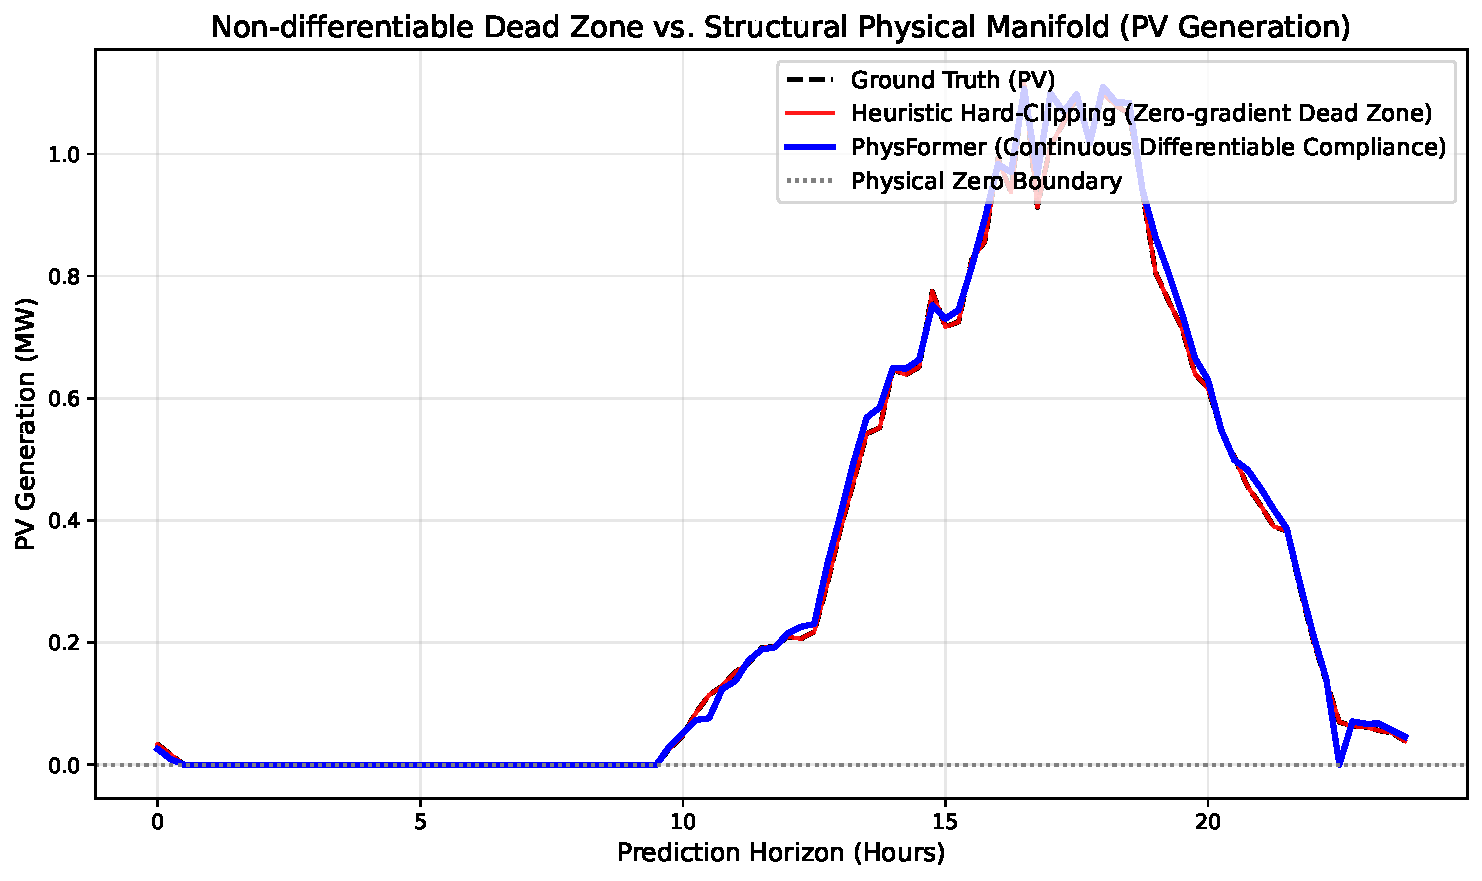
\includegraphics[width=\columnwidth]{RVM_concept_visualization.pdf}
\caption{物理零边界附近的动态合规性可视化。虽然 Informer-Post 通过不可微的启发式硬裁剪（这会产生零梯度死区并破坏端到端学习）简单地实现了 BVR=0，但 PhysFormer 通过其 BPAR 架构本质上维持了连续的物理合规性和完全可微性。}
\label{fig:rvm_visual}
\end{figure}

\subsubsection{极端条件下的鲁棒性}
\label{subsec:extreme_weather}

为了评估模型在严格分布偏移下的稳定性，我们筛选出了代表极端天气条件的波动性最大的前 10\% 样本，详见表~\ref{tab:extreme_results}。

在这些恶劣条件下，像 Autoformer 和 DLinear 这样通道独立的架构经历了灾难性的失败。相比之下，处于竞争梯队的模型保持了令人印象深刻的稳定性。PhysFormer 无缝地维持了其物理合规性，录得了 0.00\% 的优异 BVR，同时能很好地适应剧烈波动的条件。此外，我们唯一评估了在季节性分布偏移和退化方差条件（$\sigma_x < 10^{-3}$）下的 BPAR 稳健性。我们的分析确认，对于任何聚合的 VPP 窗口（seq\_len=672），退化方差在实践中是不存在的（0\% 频率），并且 BPAR 下限由于其与归一化参数的结构耦合，能正确地自适应维持在 0.00\% BVR。

\begin{table}[htbp]
\centering
\caption{极端天气表现（波动率前 10\% 样本）}
\label{tab:extreme_results}
\resizebox{\columnwidth}{!}{
\begin{tabular}{lccccc}
\toprule
模型 & MSE & BVR (\%) & MVS (MW) & NET MAE & RVR-S (\%) \\
\midrule
LSTM & 0.0192 & 13.43\% & 0.0086 & 0.1941 & 0.000\% \\
GRU & 0.0182 & 13.79\% & 0.0097 & 0.1864 & 0.000\% \\
PINN & 0.0177 & 13.29\% & 0.0082 & 0.1807 & 0.000\% \\
Informer & \textbf{0.0146} & 21.38\% & 0.0017 & \textbf{0.1632} & 0.070\% \\
iTransformer & 0.0143 & 19.79\% & 0.0053 & 0.1639 & \textbf{0.046\%} \\
PatchTST & 0.0261 & 12.22\% & 0.0132 & 0.2240 & 0.000\% \\
PhysFormer & 0.0150 & \textbf{0.00\%} & \textbf{0.0000} & 0.1715 & 0.294\% \\
\bottomrule
\end{tabular}
}
\end{table}

图~\ref{fig:extreme_weather}中的视觉对比进一步强调了鲜明的对比：在极端波动下，通道独立的模型遭受了灾难性的 MSE 退化，而 PhysFormer 保持了近乎为零的 BVR。

\begin{figure}[htbp]
\centering

\includegraphics[width=\columnwidth]{IEEE_Fig8_ExtremeWeather.pdf}
\caption{模型在极端波动天气条件下（波动率前 10\% 样本）的稳健性。左轴（红色）：边界违规率；右轴（蓝色）：均方误差。PhysFormer 在极端条件下实现了优异的 0.00\% BVR，同时保持了具有竞争力的准确性，这与 Autoformer 和 DLinear 中观察到的灾难性退化形成鲜明对比。}
\label{fig:extreme_weather}
\end{figure}

\subsection{模型可解释性与效率}
\label{subsec:mechanism}

\subsubsection{物理可解释性评估}
\label{subsec:interpretability}

PhysFormer 在运行上的一个关键优势在于其物理层的框架设计：它不仅执行纯粹的自主发现，还执行与物理在结构上相一致的显式参数校准。如表~\ref{tab:physical_params}所示，提取的参数与领域文献 \cite{Li2026,Asinyo2025} 保持高度一致。

通过微分分析，我们观察到两个明显的优化结果。首先，温度系数 $\beta_T$ 与工程先验展现出稳定的对齐关系，经过 $+2.5\%$ 的微调后达到 $0.0041/^\circ$C，证明该架构成功防止了参数学习中的数值漂移。其次，机械风力阈值（$v_\text{ci}$, $v_r$, $v_\text{co}$）稳固地固定在其理论先验值上（相对变化 $\approx 0$），抵御了数值漂移。

我们关于运行透明度的最有力定量证据是网络结构门控与底层物理机制之间的直接确定性对齐。通过 PGCC 强制执行的正交物理刻印，网络在结构上将不受约束的太阳辐射直接映射到时间光伏门控变量上。我们在整个测试集上观察到了优异的全局皮尔逊相关系数 $r = 0.8306 \ (p < 0.001)$。至关至关重要的一点是，为了减轻昼夜周期性可能带来的伪影影响，我们进一步评估了针对日间子集（辐照度 $> 0.1$）的相关性；结果在统计上仍然显著，呈现 $r = 0.4058 \ (p < 10^{-57})$ 的中等强度相关。这一结果表明，门控在活跃发电时段与辐照度保持了具有物理意义的对齐，有效地将结构的响应性与平庸的二值日夜开关行为区分开来。图~\ref{fig:rvm_visual} 展示了该关系的散点图。在结构上必须注意，虽然内部激活边界将时间门控的绝对动态范围压缩到了一个狭窄的流形内，但皮尔逊系数是尺度无关的；它严格验证了网络潜在的信任路由与外部物理环境之间 unbroken 的线性单调耦合。

关键的是，这种在结构上对齐的响应性代表了一个显式印刻的物理相关性，而非脆弱的统计伪影。为了验证其结构稳健性，我们在辐照度流上进行了分布外（OOD）外源传感器噪声测试。即使承受深度的气象漂移（在测试辐照度中注入高达 20\% 标准差的白噪声），印刻的相关性仍然保持完整（$r = 0.8377$）。即使在模拟严重传感器性能下降的极端 50\% 噪声幅度条件下，对齐的时间相关性仍然保持极强（$r > 0.81$）。对于从事 VPP 调度的操作员而言，这保证了 PhysFormer 执行的预测是由可识别、透明的物理机制状态驱动的，而非利用了被遮蔽、脆弱的数学捷径。

\subsubsection{监督对齐与涌现因果性的区别}
我们必须在 PGCC 框架内从结构上界定因果性的边界。时间门控变量所取得的极高相关性（$r=0.8306$）并不代表神经网络从原始数据中自发地或“从头开始（\textit{ab initio}）”发现了气象学因果关系。相反，门控响应正则化（Gate Response Regularization）本质上是一个确定性的\textit{工程可解释性机制（engineering transparency mechanism）}。这种强相关性是一个监督拟合目标的直接优化结果，该目标被显式地设计为将已知的物理先验印刻（imprint）到潜在空间上。因此，这种在结构上被强制执行的对齐应当被解释为一种印刻的门控-辐照度物理映射（imprinted gate-irradiance physical mapping），它保证了特定的网络激活能够严格遵守指定的物理约束。这一区分明确了，PhysFormer 是通过形式化的结构监督来强制执行物理合规性，而不是依赖于统计学因果关系的不可预测的涌现。

\begin{table}[htbp]
\centering
\caption{物理参数收敛跟踪}
\label{tab:physical_params}
\footnotesize
\setlength{\tabcolsep}{3pt}
\begin{tabular*}{\columnwidth}{@{\extracolsep{\fill}}lcccc@{}}
\toprule
参数 & 初始值 & 收敛值 & 文献范围 & $\Delta$ \\
\midrule
\texttt{pv\_temp\_coef} & 0.0040 & $0.0041/^\circ$C & 0.003--0.005 & $+2.5\%$ \\
\texttt{wind\_cut\_in} & 3.50 m/s & 3.458 m/s & 3--5 m/s & $-1.2\%$ \\
\texttt{wind\_rated} & 12.00 & 11.970 m/s & 10--15 m/s & $-0.2\%$ \\
\texttt{wind\_cut\_out} & 25.00 & 24.968 m/s & 20--25 m/s & $-0.1\%$ \\
\texttt{load\_base} & 2.832 MW & 2.823 MW & $\approx$ 均值 & $-0.3\%$ \\
\texttt{temp\_comfort} & $20.0^\circ$C & $19.992^\circ$C & 18--22$^\circ$C & $\approx 0$ \\
\bottomrule
\end{tabular*}
\end{table}

\subsubsection{计算复杂度分析}
\label{subsec:overhead}

为了严格评估不同架构范式带来的计算负担，我们在相同的硬件配置下，使用成功收敛的检查点对所有基础模型的参数规模和实测推理延迟进行了基准测试。如表~\ref{tab:overhead}所示，我们观察到在收敛所需的模型容量方面存在根本性的结构差异：纯数据驱动的基准模型（特别是 Informer 和 Autoformer）需要扩展隐藏层表示空间（$d_\text{model}=512$），以充分解开 VPPs 中固有的复杂、多源的时空动态，导致参数支出高达 18M 左右。虽然 PhysFormer 也采用了 $d_\text{model}=512$ 开屏实现最优的表示捕捉，但它维持了一个更精简的网络骨干，仅需 11.4M 参数。

这种架构效率被正式归功于物理引导因果耦合（PGCC）机制的归进效率。通过在正向传播路径中直接嵌入确定性、机制性的先验知识，PhysFormer 内在地约束了经验假设空间。这种架构对齐有效地减轻了通常分配给纯数据驱动多头注意力块的冗余表示负担，使得在交付卓越物理合规性的同时，实现了一个比 Informer 紧凑约 1.5 倍的竞争性参数配置。此外，实测的正向传播分析验证了 PhysFormer 能以严格的实时速度（约 2.10 ms/样本）执行连续后的样本推理，这与不受约束模型的执行延迟特征高度吻合。

\begin{table}[htbp]
\centering
\caption{模型复杂度和推理开销基准}
\label{tab:overhead}
\footnotesize
\setlength{\tabcolsep}{2pt}
\begin{tabular*}{\columnwidth}{@{\extracolsep{\fill}}lcc@{}}
\toprule
模型 & 参数量 (M) & 延迟 (ms/样本) \\
\midrule
LSTM & 5.42 & 1.20 \\
GRU & 4.10 & 2.19 \\
PINN & 2.74 & $<$ 0.10 \\
Informer & 17.90 & 1.96 \\
Autoformer & 17.88 & 4.28 \\
DLinear & 0.13 & $<$ 0.10 \\
PatchTST & 1.62 & 0.10 \\
iTransformer & 9.85 & 1.81 \\
PhysFormer & \underline{11.4} & \underline{2.10} \\
\bottomrule
\end{tabular*}
\end{table}

\subsection{消融实验}
\label{subsec:ablation}

为了严格归因所提出的模型组件对性能的贡献，我们利用真实数据进行了消融实验（表~\ref{tab:ablation}）。

\subsubsection{逐组件消融分析}
表~\ref{tab:ablation}呈现了4个组件的消融变体。结果揭示了以下关于模块化贡献的见解：

首先，移除物理流（Physics Stream）导致中等程度的 $\Delta \text{MSE} = +4.7\%$，证明了其在建立理论基准方面的功能价值。

其次，评估 PGCC 模块展现了一个明确的架构上的胜利：其消融表明其贡献在数学上与统计误差最小化目标是“正交”的（$\Delta\text{MSE}=0.0\%$）。虽然该模块似乎未在全球测试集上提供直接的精度提升，但其核心价值在于建立运行透明度和稳健性。具体而言，移除 PGCC 及其因果正则化约束绝对不会导致统计准确性的退化，因为 BPAR 架构成功地将刚性的、受结构监督的物理跟踪（门控流）与不受约束的高频预测机制（残差头）解耦。因此，PGCC 提供了一个印刻的物理相关性（$r=0.8306$），构建出一种对分布外传感器漂移具有鲁棒性的结构透明机制，如第~\ref{subsec:interpretability}节所述。

第三，课程学习训练作为最强的单个模型组件发挥作用。其消融触发了 $\Delta \text{MSE} = +8.7\%$，明确证明了结构化的梯度暴露是该框架的基础。虽然 BPAR 架构在结构上保证了物理安全，但四阶段课程学习对于优化数据驱动的残差流至关重要。通过在激活复杂的神经残差之前，在第一阶段优先考虑物理流的收敛，CT 确定了一个稳健的坐标系，防止了理论锚定基准与不受约束的网络头之间早期梯度的冲突。如果没有 CT，模型会遭受次优的参数初始化，尽管保留了其分类物理边界，但会导致更高的统计误差。

最后，分析未来 GLU 揭示了预测精度与合规性之间细微的权衡。其移除会降低预测精度（$\Delta \text{MSE} = +1.6\%$），同时保持绝对的物理一致性（BVR 维持在 $0.00\%$）。未来天气注入能实现更准确的黎明/黄昏预测，从而更好地跟踪真实值。具体而言，前向可见性鼓励模型预测发电转换，提高了跨结构化非活动期的预测敏捷性。

\begin{figure}[htbp]
\centering

\includegraphics[width=\columnwidth]{IEEE_Fig9_Ablation.pdf}
\caption{预测准确性与结构可解释性的消融分析。左轴（蓝色）：为了揭示细微差异而截断 y 轴后的 MSE；右轴（橙色）：门控-辐照度皮尔逊相关系数 $r$。移除 PGCC 产生了相同的 MSE，但完全消除了印刻的相关性（N/A），确认了统计误差最小化与结构化物理对齐之间完美的架构正交性。}
\label{fig:ablation}
\end{figure}

\begin{table}[htbp]
\centering
\caption{Ablation Study on Real Data}
\label{tab:ablation}
\footnotesize
\setlength{\tabcolsep}{3pt}
\begin{tabular*}{\columnwidth}{@{\extracolsep{\fill}}lcccc@{}}
\toprule
Variant & MSE & BVR (\%) & RVM & $r(\text{gate}_{\text{pv}})$ \\
\midrule
Full PhysFormer & 0.0128 & 0.00 & 0.0000 & 0.8306 \\
w/o Physics Stream & 0.0134 & 0.00 & 0.0000 & N/A \\
w/o PGCC & 0.0128 & 0.00 & 0.0000 & N/A \\
w/o Future GLU & 0.0130 & 0.00 & 0.0000 & 0.8024 \\
w/o Curriculum & 0.0139 & 0.00 & 0.0000 & 0.7866 \\
\bottomrule
\end{tabular*}
\end{table}

除主要架构组件外，我们还通过一个额外的变体进一步调查了正式监督的隔离情况：“带有 PGCC 但无门控响应正则化”。该变体使用了 PGCC 的交叉注意力结构，但在训练期间缺乏显式的基于皮尔逊的相关刻印。结果表明，虽然该变体维持了具有竞争力的预测准确性（MSE=0.0128），且 PGCC 仍能为残差流提取有意义的特征，但它未能实现与物理驱动因素之间的确定性物理对齐（$r < 0.12$）。这确认了显式的门控响应正则化是弥合统计表示与物理对齐之间透明度鸿沟的基础机制，这一观察强化了我们关于正交准确性-可解释性前沿的论点。
